%%% -*-LaTeX-*-

\chapter{SweetPea Language}

SweetPea achieves its goal of creating unbiased experimental sequences from high-level experimental designs by relying on a SAT sampler. Writing experimental designs in the language of a SAT sampler-- that is, as a boolean formula-- is, at best, highly uncomfortable. SweetPea, therefore, conveniently bridges the gap between scientists and SAT samplers: scientists describe their experimental designs in the terms they usually use in their domain, and SweetPea handles the rest.

In this chapter, we'll document the features of the SweetPea language. They largely follow the components we saw in the Overview chapter. Experimental design specifications consist of:
\begin{itemize}
  \item trials described in terms of factors and levels,
  \item constraints and relationships over those trials,
  \item counting and balancing constraints,
  \item and a block specification consisting of a crossing and a design.
\end{itemize}

Here we'll look at a variety of experiments which motivate these various features, and the high-level language we provide to describe those experiments. In the next chapter we'll take a close look at how these features are efficiently encoded into a boolean formula.


\section{Experimental Design Wishlist}

We briefly saw the parts of an experiment with the Stroop test in Chapter 2. Now let us look at the range of variations of trial-based experiments we might wish to model.

\subsection{Descriptions of Stimuli}

Each component of a stimulus is represented as a \emph{factor} which typically takes on a discrete number of \emph{levels}. In the Stroop experiment there were two factors (display color and text) each with two levels (red and blue). A typical experiment have 2 to 7 factors with 2 to 4 levels each, resulting in roughly 50 to 200 stimuli.

Levels may be nested into sub-levels. One reason for doing so is to apply different constraints to each of the sublevels. For instance, a color factor may have nested sublevels of light colors (like yellow and aqua) and dark colors (like navy and maroon).

Sometimes researchers may want to define factors with levels sampled from a continuous distribution, for example to model a spectrum of light or sound. Sweetpea currently does not support this other than by the researcher manually discretizing the continuum into several discrete values. This case is particularly challenging for SweetPea because it is difficult to phrase sampling a continuous distribution as a boolean formula; for more thought on how we could better support this see Future Work.

\subsection{Ordering Constraints}

Researchers must have some control over the ordering of stimuli to be able to test their hypothesis. For example, if we are testing whether the presence of a certain level affects the participant's reaction time, we need control over when that level occurs and how often it occurs in relation to other levels. More generally, we need to be able to constrain the presence or absence of relationships which we define over the levels. Since levels can be grouped into arbitrary sub-levels, we should more generally be able to specify constraints on relationships over the sub-levels.

One example of such a relationship is a transition constraint, which specifies whether each level is followed by the same level (a repetition) or a different level (a switch). This is an important condition to control for in task-switching experiments because a participant's reaction time may depend on whether they just performed a similar or dissimilar task. An experimenter may wish to specify that a participant experience as many repetition or tasks as task switches.

Another example, which we saw in Chapter 2, is a congruence constraint, which specifies whether the levels of different factors are, according to a user-specified condition, complementary or conflicting. A congruence constraint for the Stroop test is whether the text and the color it is displayed in are the same (the word "red" displayed in red) or not.

Constraints can also be defined in terms of other constraints. For instance, in the Stroop test one may want to balance the number of congruent and incongruent levels, or to balance the transitions between congruent and incongruent levels. More generally, experiments expressed in SweetPea may need to define user-specified relationships between levels.

\subsection{Experimental Design and Balancing}

Experiments which include every possible combination of levels are fully crossed designs. Full crossings are desirable because they allow the researcher to test the full space of possible stimuli.

Sometimes, however, factors either need to be excluded or duplicated to make an experiment feasible. For example, a participant can only reliably be tested for so long before they are tired, so sometimes factors which are deemed to be irrelevant to the control variables and variables of interest are excluded from the full crossing. If an experiment is too large it can either be restated as a full crossing of only a subset of the factors (with the non-crossed factors being assigned at random, with uniform probability), or it can be divided across participants or across experimental sessions. An experiment can be too small if the full crossing has too few stimuli to reliably draw conclusions. In this case, the experiment can either be multiple full crossings back-to-back, or the contents of multiple full crossings combined into a larger experimental block.

Fully-crossing a design is a form of balancing-- it is the specification that each level occurs as frequently as each other level, that each level occurs once, and that all combinations of levels occur with equal frequency.

\begin{figure}[t]
    \centerline{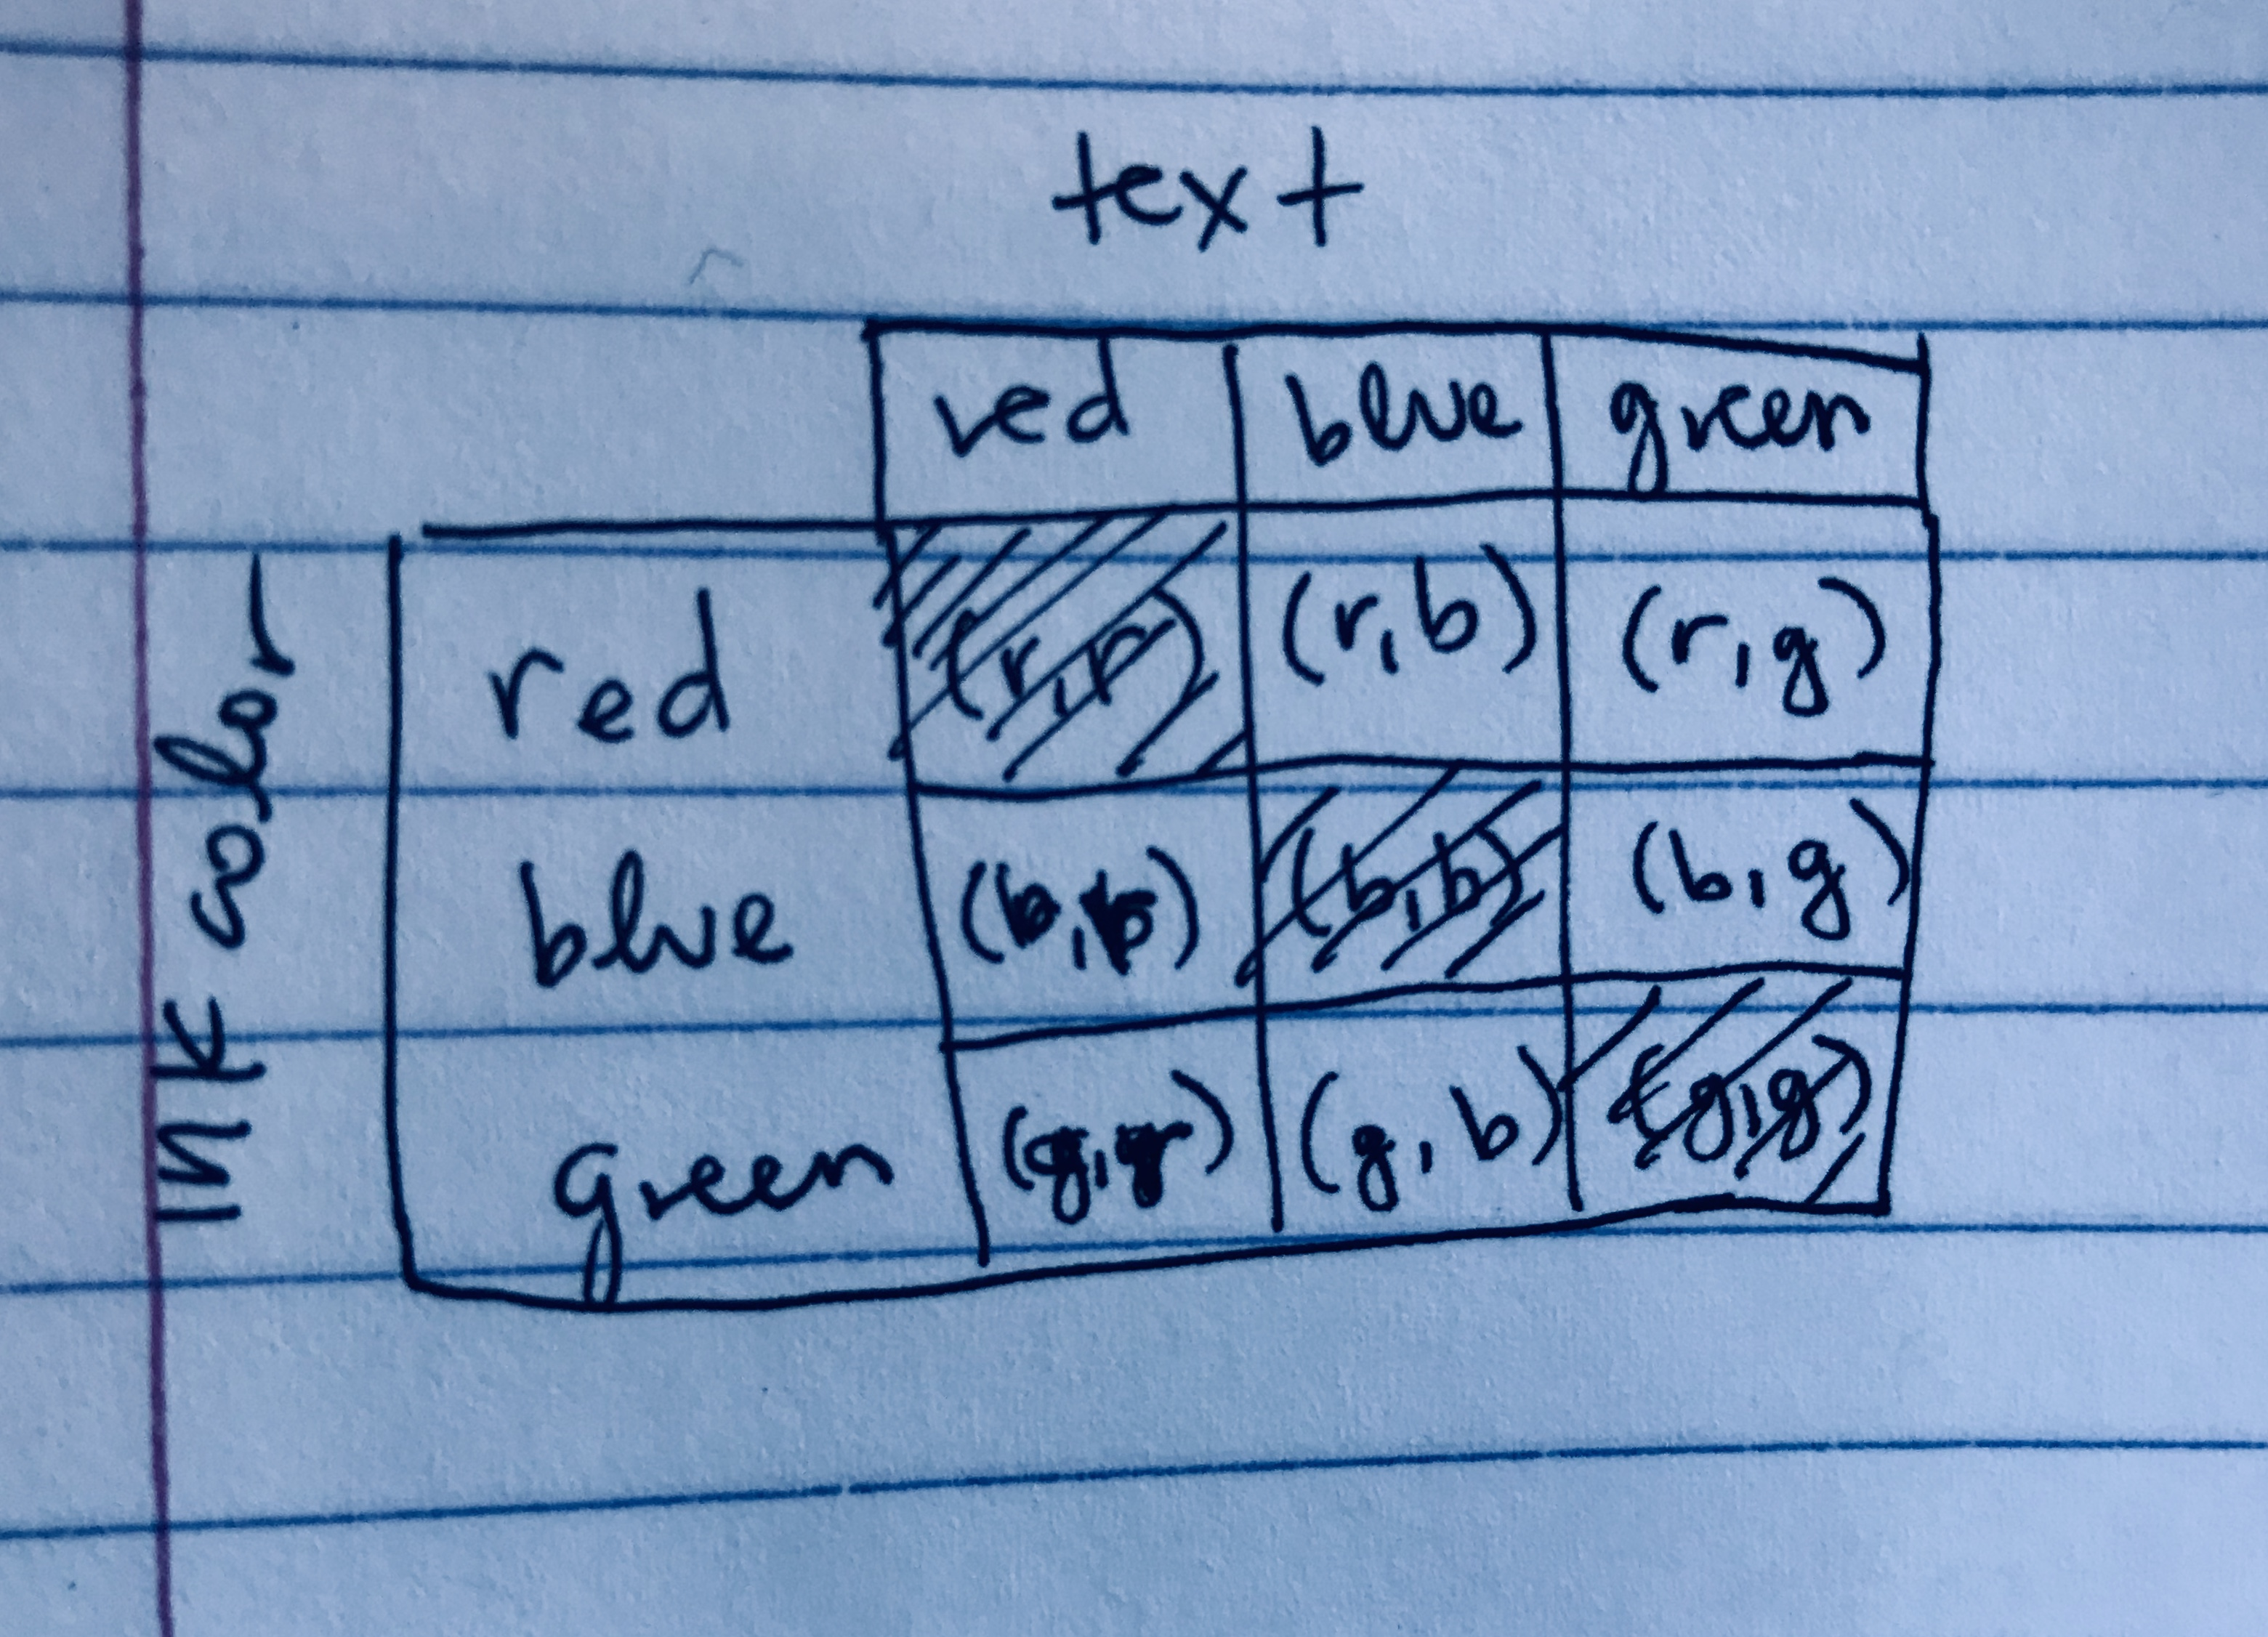
\includegraphics[origin=c,width=10cm]{fig_weighted_crossing}}
    \caption{Full crossing of a 3 color Stroop experiment. There are more congruent stimuli (along the diagonal) than incongruent stimuli.}%
    \label{fig:weighted_crossing}%
\end{figure}

Sometimes the constraint of using a full-crossing makes other types of balancing impossible because the levels are over-constrained. Consider, for instance, the Stroop test with 3 different colors instead of two (as in \figref{weighted_crossing}): then it isn't possible to both fully-cross the design and to balance the congruent and incongruent levels. (This is because there are 3 congruent levels, and 6 incongruent levels). One possible desired outcome in this case is for SweetPea to report that an experiment is over-constrained.

Another alternative is that if balancing the congruent and incongruent levels is more important than a fully-crossed design, then we can instead create a \emph{weighted crossing}. In a weighted crossing we can specify that we wish to under-sample certain levels (the incongruent ones in our example) or over-sample other levels (the congruent ones). Weighted crossings also allow us to express the experiments mentioned above, where the full crossing has either too many or too few stimuli to be practical. This desirable, more general crossing specification, is not currently implemented in SweetPea and is further discussed in the Future Work Chapter.

\subsection{Structure of an Experiment}

An experiment is composed of one or more experimental blocks; an experimental block is a sequence of stimuli. Experiments may be organized into blocks for several reasons: there may be prologue or epilogue blocks which set up some condition for the participant, the experiment may be designed to be run in several related sessions, or consist of several sub-experiments.

It is not always possible to balance some commonly desired constraints with a single block; for instance, it is not possible to have as many "repeat" transitions as "switch" transitions in the fully-balanced Stroop experiment because there are an even number of stimuli, resulting in an odd number of transitions. This means it is not possible to have exactly as many of one transition as the other.

There are two approaches to resolving this issue. The first is nearly-balancing the levels: instead of requiring that there are exactly the same number of each level, require that there are the same number plus-or-minus one. The other solution is to create a "throw-away" block with a single stimulus in it which is used to satisfy the transition balancing constraint without being included in the full-crossing constraint.

As mentioned in the previous section, it is also sometimes useful to have multiple blocks to repeat stimuli for an experiment with too few stimuli or to break up an experiment with too many stimuli across several sessions or participants.

\section{SweetPea Language Reference}

Now that we have the context of the types of experiments we would like to model, let us discuss the SweetPea grammar. A specification of an \texttt{Experiment} is a valid SweetPea program. The full schema is provided below; each part will be discussed in detail and each term defined in the following subsections:

\begin{verbatim}
Experiment         = [Block, ...]
Block              = Design Crossing [Constraint, ...]
Design             = [Factor, ...]
Crossing           = [Factor, ...] CrossingType
CrossingType       = FullyCrossed
                   | MultipleFullyCrossed
Constraint         = AtMostKInARow  K (FactorName, LevelName)
                   | ExactlyKInARow K (FactorName, LevelName)
                   | AtLeastKInARow K (FactorName, LevelName)
Factor             = FactorName [Level, ...]
                   | FactorName [DerivedLevel, ...]
DerivedLevel       = LevelName Window
Window             = Stride Width DerivationFunction [FactorName, ...]
DerivationFunction = ( [FactorName, ...]... ) -> Boolean
Level              = <any printable type> | [Level, ...]
FactorName         = <any printable type>
\end{verbatim}

Some of these terms are specified directly, like FactorName and Level, while others are created via constructors. A full list of the constructors in SweetPea is:

\begin{verbatim}
Factor constructor:
  Factor(<factor name>, <list of levels>)

Window constructors:
  Transition(<derivation function>, <list of factors>)
  WithInTrial(<derivation function>, <list of factors>)
  Window(<stride>, <width>, <derivation function>, <list of factors>)

DerivedLevel constructor:
  DerivedLevel(<level name>, <window>)

Counting Constraint constructors:
  AtMostKInARow (<k>, (<factor name>, <level name>))
  ExactlyKInARow(<k>, (<factor name>, <level name>))
  AtLeastKInARow(<k>, (<factor name>, <level name>))

Block constructors:
  FullyCrossBlock(<design>, <crossing_factors>, <weights>)
  MultipleFullyCrossBlock(<design>, <crossing_factors>, <weights>, <numReps>)
\end{verbatim}

Once the user has constructed a complete SweetPea specification by creating an \texttt{Experiment}, they can call a function to synthesize the experimental sequence:

\begin{verbatim}
synthesize_trials(<experiment>, <number of experiment sequences>)
\end{verbatim}

The remaining subsections will investigate and document each component of the grammar.

\subsection{Factors and Levels}

\begin{verbatim}
  Factor             = FactorName [Level, ...]
                     | FactorName [DerivedLevel, ...]
  Level              = <any printable type> | [Level, ...]
  FactorName         = <any printable type>
\end{verbatim}

Factors are constructed as named tuples, specified by factor names, and a possibly nested list of levels, each of which also has a name. Names are used to specify the experimental sequence that the runtime eventually returns, but they do not need to be strings. They can be any "printable" data-type; this can be useful because names are referenced in user-defined constraints as we'll see in the next subsection.

\begin{verbatim}
example_factor = Factor("example_name", ["example_level"])
boolean_factor = Factor("booleans",     [False, True])
numeric_factor = Factor(1234,           [1, 2, 3, 4])
text           = Factor("text",         ["red", "blue"])
light_colors   = Factor("light_colors", ["yellow", "aqua"])
dark_colors    = Factor("dark_colors",  ["navy", "maroon"])
display_color  = Factor("display_color",    [light_colors, dark_colors])
\end{verbatim}

In the resulting experimental sequence, exactly one choice of level is selected per trial; if a factor has nested levels then the nesting is flattened in the final experimental sequence. Nesting is only useful at the high-level to describe groupings of levels, for instance to be the participant of a constraint.

\begin{figure}[t]
    \centerline{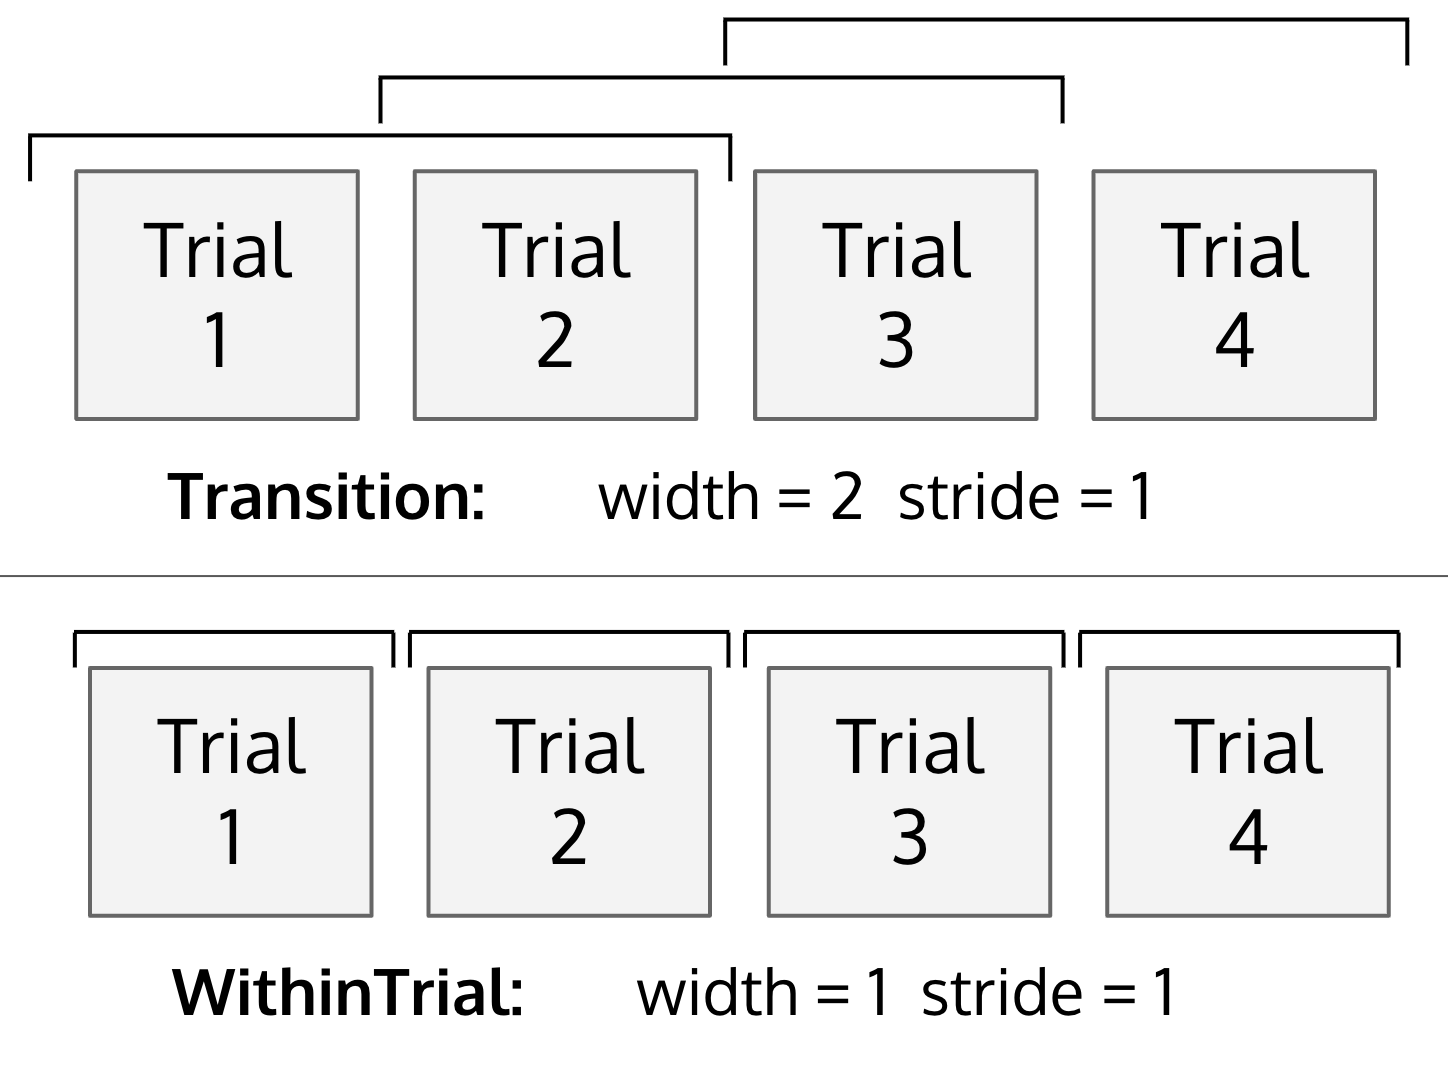
\includegraphics[origin=c,width=10cm]{fig_windows}}
    \caption{Windows define the scope of relationships between trials.}%
    \label{fig:windows}%
\end{figure}


\subsection{Deriving Levels with Windows}

\begin{verbatim}
  DerivedLevel       = LevelName Window
  Window             = Stride Width DerivationFunction [FactorName, ...]
  DerivationFunction = ( [FactorName, ...]... ) -> Boolean
\end{verbatim}

How do we represent relationships between levels and enforce constraints over them? For the types of experiments that can be specified in SweetPea, all of the constraints relate to order, so let us consider a symbolic window which slides over the list of trials. A window has a width and a stride. The width specifies how many trials to consider at once; the stride specifies how many trials by which to move forward when the window moves. When combined with user-defined derivation functions, windows allow the user to specify new "derived" levels and factors based on the values of the levels within the window. We will see two examples of this shortly.

SweetPea provides constructors for two common window sizes: \texttt{WithinTrial} windows, which are used to define new properties based on properties of each individual trial have width of 1, stride of 1. \texttt{Transition} windows, which are used to define properties based on each consecutive pair of trials, have width of 2, stride of 1.

\begin{verbatim}
  Window Constructors:
Transition(<derivation function>, <list of factors>)
WithInTrial(<derivation function>, <list of factors>)
Window(<stride>, <width>, <derivation function>, <list of factors>)
\end{verbatim}

Consider the transition relationship, which for a given factor specifies whether each following trial has the same value for that factor (a repetition) or a different value (a switch). We will represent this relationship as a new, derived, factor. This factor has two levels: one level which indicates that the following stimulus was a repetition, and the other that it was a switch. What are the parameters for the window for this relationship? Because we consider two trials at a time, and want to consider all pairs of consecutive trials, the width is two, and the stride is one.

Given this conceptual window, the user can then provide a function for each derived level of the derived factor which specifies, based on the values of the levels which are "in scope" in the window, whether the derived level is selected or not. For the transition example, this may look like:

\begin{verbatim}
def repetition(display_colors):
  if display_colors[0] == display_colors[1]:
    return True
  return False
\end{verbatim}

The repetition function takes a list of display colors. Because we're considering all consecutive pairs of trials, the window size is two, so the length of the display colors list is also two. Conceptually, this function will be applied to all consecutive pairs of trials and report whether those trials are repeat or not.

We can use this repetition function to define a new pair of levels. Recall that levels act as indicators; when a level of a trial is true, that means that trial possesses the quality that level represents. The level derived using a transition-wide window and the repetition function defined above is true when the trial is has the same display color property as the trial before it. Because levels can be defined to be any [printable] type, derivation functions can use any property of the level name as part of their logic.

Putting it all together, in the running example, these derived levels are represented in SweetPea as:

\begin{verbatim}
display_color = ("display_color", ["red", "blue"])
text      = ("text",      ["red", "blue"])

def repetition(display_colors):
  if display_colors[0] == display_colors[1]:
    return True
  return False

def switch(display_colors):
  return not repetition(display_colors)

repeat_level = DerivedLevel("repeat",
                 Transition(repetition, [display_color]))
switch_level = DerivedLevel("switch",
                 Transition(switch, [display_color]))
transition_factor = Factor("transition?", [repeat_level, switch_level])

\end{verbatim}

Let us consider another use-case. A central factor of a Stroop experiment is whether the text and the color it is displayed in specify the same color or not. We can define this relationship by considering a \texttt{WithinTrial} window, in which the width is one (since we consider a single trial at a time), and the stride is also one. The derivation function for congruence is similar to the one for repetitions; here however we always compare the first (and only) item in the display colors and texts lists.

\begin{verbatim}
display_color = ("display_color", ["red", "blue"])
text      = ("text",      ["red", "blue"])

def congruent(display_colors, texts):
  if display_colors[0] == texts[0]:
    return True
  return False

def incongruent(display_colors, texts):
  return not congruent(display_colors, texts)

con_level  = DerivedLevel("con",
               WithinTrial(congruent, [display_color, text]))
inc_level  = DerivedLevel("inc",
               WithinTrial(incongruent, [display_color, text])
congruence_factor = Factor("congruent?", [con_level, inc_level])
\end{verbatim}

Windows allow us to represent, more generally than just transitions and within-trial constraints, relationships across a sequence of trials. See \figref{windows} for an illustration. Some experiments may wish to define relationships which skip trials in the middle of the sequences. Another example is an experiment with a "bait" trial: participants are asked to respond based on a property of a trial some number of trials previous. Additionally, changing the stride allows for things like specifying a constraint over the first half, and then second half of the experiment.

SweetPea currently supports transition and congruency constraints, but does not support the most general form of derivation function. See future work for a discussion on how to handle fully arbitrary derivation functions.

\subsection{Counting Constraints}
SweetPea also provides three counting constraint constructors which let the user constrain levels to appear some number of times. These constructors are also named tuples, which take the number to count to, k, and the level to which apply this constraint. Since individual levels are not directly referenced by variables, the user must specify a tuple of factor name and level name.

\begin{verbatim}
Counting Constraint constructors:
  AtMostKInARow (<k>, (<factor name>, <level name>))
  ExactlyKInARow(<k>, (<factor name>, <level name>))
  AtLeastKInARow(<k>, (<factor name>, <level name>))
\end{verbatim}

The \texttt{AtMostKInARow} constraint is useful as a "sanity check" constraint, to ensure that independent variables do not show up an unreasonable number of times.

\subsection{Experimental Design, Balancing and Experimental Structure}

\begin{verbatim}
Experiment         = [Block, ...]
Block              = Design Crossing Constraints
Design             = [Factor, ...]
Crossing           = [Factor, ...] CrossingType
CrossingType       = FullyCrossed
                   | MultipleFullyCrossed
Block constructors:
  FullyCrossBlock(<design>, <crossing_factors>, <weights>)
  MultipleFullyCrossBlock(<design>, <crossing_factors>, <weights>, <numReps>)
\end{verbatim}

Once we have described the trials in terms of levels and factors, we need to specify the set of trials that make up the experiment. The design of the experiment is the specification of factors which represent a trial. To specify the set of trials in the experiment we need to specify the crossing of the design. As mentioned before, a full crossing is commonly, but not always, used.

The design is specified explicitly as a list of factors, while the block is built by a constructor which knows how to construct the block based on the crossing type. Each constructor takes two lists of factors, one which represents all the factors relevant to a trial (\texttt{design}), and one which represents which factors should be included in the crossing (\texttt{crossing\_factors}). Each trial in the resulting experimental sequence will have a value for factors specified in \texttt{design}.

The final aspect we need to specify is the structure of the experimental sequence. An experimental sequence is a list of one or more experimental blocks. Each experimental block consists of a crossing of the experimental design. Some experiments may wish to specify multiple experimental blocks to represent prologue or epilogue blocks, or to split an experiment across multiple sessions.

Finally, to generate the experimental sequence, the user can call \texttt{synthesize\_experiment} which takes an \texttt{Experiment} and produces a list of trial specifications.

Putting together all the code snippets in this section, here is a full specification of a simple Stroop experiment in SweetPea:

\begin{verbatim}
display_color = ("display_color", ["red", "blue"])
text      = ("text",      ["red", "blue"])

def congruent(display_colors, texts):
  if display_colors[0] == texts[0]:
    return True
  return False

def incongruent(display_colors, texts):
  return not congruent(display_colors, texts)

con_level  = DerivedLevel("con",
               WithinTrial(congruent, [display_color, text]))
inc_level  = DerivedLevel("inc",
               WithinTrial(incongruent, [display_color, text])
congruence_factor = Factor("congruent?", [con_level, inc_level])

design       = [color, text, conFactor]
crossing     = [color, text]

constraints = [NoMoreThanKInARow(1, ("congruent?", "con"))]

block        = FullyCrossBlock(design, crossing, constraints)

experiments  = synthesize_trials(block, 5)
\end{verbatim}

This design will produce an experimental sequence which might look like:

\begin{verbatim}
color blue | text red  | congruent? inc
color blue | text blue | congruent? con
color red  | text blue | congruent? inc
color red  | text red  | congruent? con
\end{verbatim}


In this chapter we have seen the SweetPea language features, which is the information a user would want to program in SweetPea. We have not yet discussed how these language features are implemented; in the following two chapters we will see how each of these primitives is encoded as a part of a boolean formula.
